
In embedded, IoT class devices to which an attacker may have
physical access,
Differential Power Analysis (DPA) attacks on cryptographic implementations
\cite{KJJ:99} can be devastating.
DPA attacks rely on the power consumption of an attacked device being
corrolated with secret values (i.e. cryptographic keys) being manipulated.
By observing the power consumption of the device while processing
attacker controlled inputs (plaintexts), one can model the {\em expected}
power consumption based on simple hamming-weight or hamming-distance
calculations of expected instruction results.
The secret value is recovered by correlating the predicted power
consumption with the observed traces.

While ISEs give a notable increase in efficiency, they can also create
attractive targets for DPA attacks.
This stems from there being only one way to sensibly implement
AES using the ISE, thus reducing the number of target variables an
attacker needs to consider.

Having identified ISE \ISE{3} as a strong standardisation candidate
for embedded $32$-bit RISC-V cores, we now show a possible
way of extending the ISE further to add 
$1$'st order DPA side-channel resistance.

\subsection{Design and implementation}

We base our design on boolean-masking, and represents the secret
key as two boolean masked shares.

An implementation of the AES block encrypt/decrypt function 
using \ISE{3} requires eight registers:
four for the current round state,
four to load the next round key into and then accumulate the next round state.
See \REFFIG{fig:v3:round} for an AES round function implementation
using \ISE{3}

Storing shares of each secret variable
in the General Purpose Register (GPR) file is un-reasonable.
It would require drastic modifications to the instruction definitions and
register file to read four registers (two sources, of two shares each) and
write two registers.
While this is not insurmountable for a more general purpose ISE
(especially where adjacent register pairs are used to store corresponding
shares),
it would break the RISC-V $2$-read-$1$-write principle.
Storing corresponding shares in the GPRs is also a security
risk, as they may be accidentally combined due to
careless instruction use, or implicit register accesses by the
CPU micro-architecture.

Instead, we define a new, $8$-element ``Mask Register File'' (MRF).
Each mask register $M_i$ is $w=32$-bits wide, and stores the mask for
one of the GPRs.
We use a fixed mapping between GPRs and mask registers;
not all GPRs have a corresponding mask register.
We use the mapping $\{a0..a3,t0..t4\} \Rightarrow \{m0..m7\}$.

Share $0$ of each secret value is loaded into the GPRs using the
standard RISC-V Load Word ({\tt lw}) instruction.
We define a new Load Mask instruction {\tt lm rd, imm(rs1)} which
loads {\em the mask for GPR {\tt rd}}
(i.e. Share $1$)
from memory into the corresponding MRF entry.
A corresponding Store Mask instruction {\tt sm rs2, imm(rs1)} writes
the mask corresponding to GPR {\tt rs2} to memory.
The {\tt sm} instruction is only used for context switches, and
destructively reads the MRF register value to prevent it being
leaked to other applications running on the same core.\footnote{
    In this case, destructive could mean set to zero (which could
    leak the hamming weight of the mask) or randomising it's value.}
We require the secret values be stored in shared form in memory
(rather than splitting them into shares upon being loaded)
to extend the SCA protection boundary outside the CPU.
Otherwise, the hamming weight of un-masked secret values would be
leaked by memory-hierarchy registers outside the CPU.
Executing an {\tt lm} instruction such that {\tt rd} does not map to
a mask register raises an illegal opcode exception.
Likewise for {\tt sm} and {\tt rs2}.

When an ISE instruction is executed and its GPR source
registers map to an MRF register, both GPR and MRF are
read simultaneously and fed to the AES functional unit.
If any GPR source does not map to an MRF register, we assume that
operand is un-masked and represent the other share as $0$.

Within the AES FU the instruction result is computed entirely in it's
masked representation.
The result shares are then re-masked before being written back to the
GPRs and MRF.
This is necessary, because \ISE{3} instructions are designed
such that {\tt rs1=rd} for all use cases.
Without re-masking, overwriting a source with the result could cause 
$1$'st order hamming-distance leakage.

If the destination GPR has a corresponding
mask register, share $0$ is stored in the GPRs and share $1$ in the MRF.
If the destination GPR does not map to a mask register, the result is written
to the GPR un-masked.
This means that in the final encrypt/decrypt round, we can obtain
the un-masked results without having to store the shares to memory,
load them back and un-mask them.

We used the \CORE{2} core as the basis for our side-channel secure
implementation of \ISE{3}.
\REFFIG{fig:core:2:secure} shows a block diagram of the modifications
made to the core, and which data-paths carry masked data.
To avoid accidental un-masking of the two shares,
Share $1$ is stored in {\em bit-reversed} form in the MRF and pipeline
stage registers.
This means that any accidental multiplexing between pipeline operand
registers causes toggles between non-corresponding bits of each share.
Share $1$ is only un-reversed immediately prior to entering the
AES functional unit, and is re-reversed before exiting it.
Bit-reversal has zero logic gate cost, but adds some minor routing
complexity.

While the architectural state stores a $2$-share representation
of the secret material, we use a $3$-share implementation of the
AES S-box.
This was driven by experiments showing 
leakage from a $2$-share design in our FPGA platform.
The additional share is generated by a simple $32$-bit LFSR and added
dynamically by the hardware, and is never visible to the programmer.
This is suitable for a proof of concept (evident in the experimental
results) but would need to be used in conjunction with a true random
number source (E.g. a set of ring-oscillators) in a deployed system.
Only the S-box is implemented using $3$-shares.
Subsequent \AESFUNC{MixColumns} logic is only implemented using $2$ shares.

\subsection{Evaluation}

We used a standard experiment plaform to evaluate the power side-channel
hardened AES \ISE{3} instructions.
The modified \CORE{2} core was implemented on a
Sasebo GIII \cite{HKSS:12}
side-channel analysis platform, containing two Xilinx FPGAs:
a Kintex-7 
(model {\tt xc7k160tfbg676})
target
and
a supporting Spartan-6
(model {\tt xc6slx45}).
Only the Kintex-7 was used.
The design was synthesised using Xilinx Vivado 2019.2 with
default synthesis and implementaiton strategies.
No effort was spent on optimising the synthesis or routing.
The Kintex-7 FPGA uses a 200MHz differential external clock source, which is
transformed into a 50MHz internal clock used by the entire
design.

Trace capture uses a standard pipeline of components:
a MiniCircuits BLK+89 D/C blocker,
an Agilent 8447D amplifier (with a $\SI{100}{\kilo\hertz}$ to $\SI{1.3}{\giga\hertz}$ range, and $\SI{25}{\decibel}$ gain),
and
a  PicoScope 5000 series oscilloscope.
The oscilloscope uses a 250 MHz sample rate, with a 12-bit resolution.
The capture process is coordinated using a laptop.

We performed a generic Test Vector Leakage Assessment (TVLA) \cite{TVLA}
flow to evaluate
the effectivness of the side-channel hardened implementation;
using the AES-128 block encrypt function as the target operation.
The un-protected and protected implementation results are shown in
\REFFIG{fig:sca:unprotected} and
\REFFIG{fig:sca:protected} respectivley.
The protected implementaiton is effective at removing $1$'st
order side-channel leakage upto $100$K traces.
The peaks at the beginning and end of \REFFIG{fig:sca:protected}
are caused by the un-masked block input and output data being loaded/stored.

\REFTAB{tab:sca:sw-hw} show the impact on hardware and software cost
of the side-channel hardening.
The ISE Size/LTP rows are inclusive of the S-box Size/LTP rows.
Likewise, the CPU Size rows are inclusive of the ISE Size rows.
For software, the static code size and executed instructions overheads are
$~20\%$; considerably less than a non-ISE based software masking approach.
The hardware overheads are dominated by the increased size of the
S-box (owing to the 3-share design), and the MRF.
Although the overhead to the dedicated
ISE logic is $~4x$, this drops to $~1.2x$ when the entire
CPU sub-system is considered.
In the context of an entire SoC, the additional logic requirements
are modest when compared with a dedicated masked AES accelerator.

\begin{table}[]
\centering
\begin{tabular}{lrrr}
Metric  & Un-protected & Protected  & Overhead \\
\hline
Static Code Size      & 290         & 358    & $1.23\times$x        \\
Instructions Executed & 238         & 287    & $1.21\times$x        \\
CPU Clock Cycles      & 291         & 331    & $1.14\times$x        \\
S-box Size (NAND2)    & 554         & 3245   & $5.86\times$x        \\
S-box LTP             & 19          & 22     & $1.16\times$x        \\
ISE Size (NAND2)      & 1157        & 4616   & $3.99\times$x        \\
ISE LTP               & 30          & 37     & $1.23\times$x        \\
CPU Size (NAND2)      & 38610       & 45141  & $1.16\times$x        \\
CPU Size  LUTs        & 4017        & 4956   & $1.23\times$x        \\
CPU Size  FFs         & 2078        & 2420   & $1.16\times$x        \\
Timing Slack @50MHz   & 8.12ns      & 7.05ns & $0.87\times$x
\end{tabular}
\caption{
Software and hardware overheads for the protected ISE implementation
of AES-128 block encryption.
The ``ISE Size'' row does not include the cost of the mask register file
for the protected implementation.
This is included in the CPU size measurements, since the exact method
of mask delivery and storage is an implmentation option.
}
\label{tab:sca:sw-hw}
\end{table}

\begin{figure}
\centering
\begin{subfigure}[t]{0.95\textwidth}
\centering
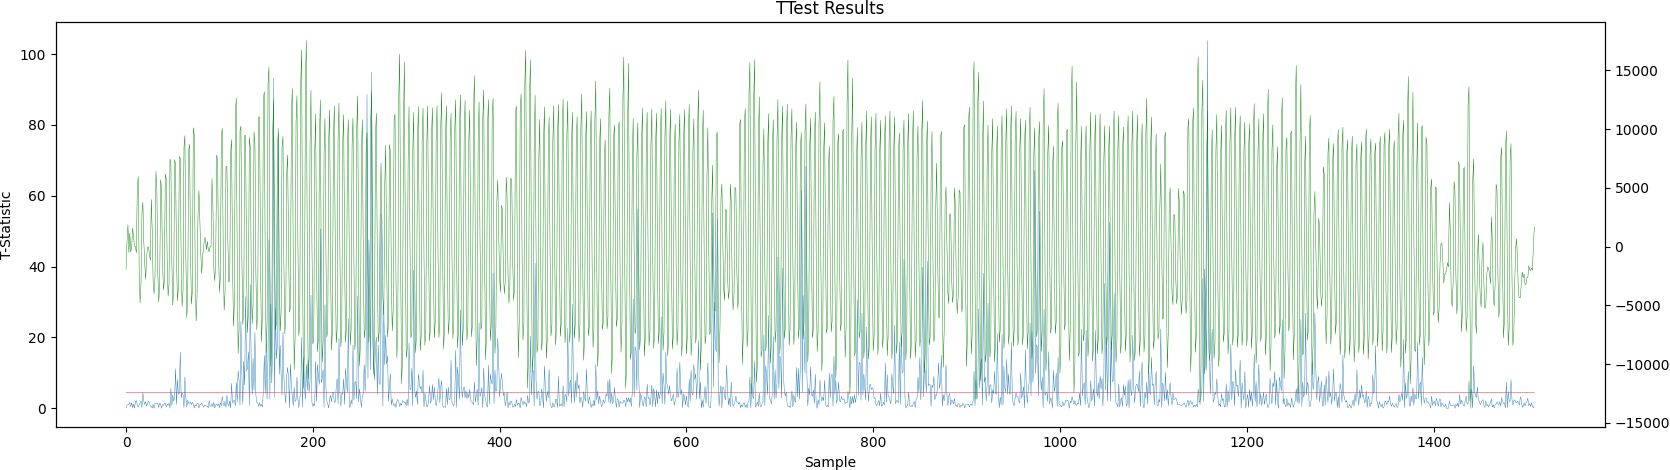
\includegraphics[width=\textwidth]{graphs/aes-vanilla-enc-default-ttest.png}
\caption{
    Un-protected implementation TVLA results after $10$K traces.
}
\label{fig:sca:unprotected}
\end{subfigure}
\begin{subfigure}[t]{0.95\textwidth}
\centering
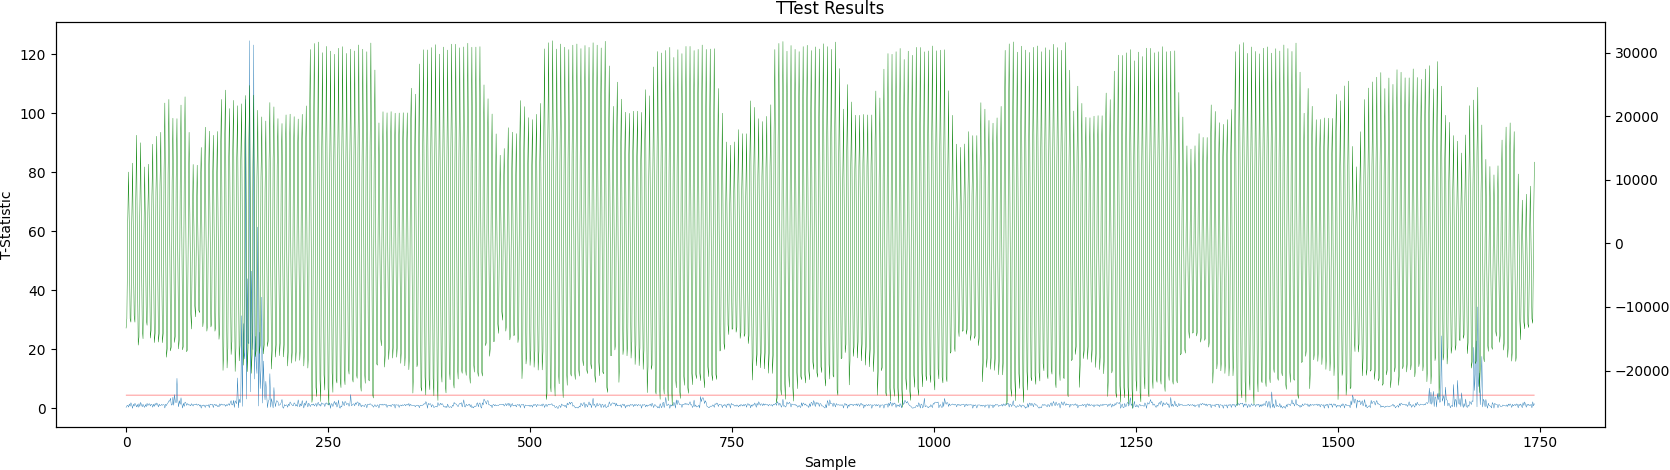
\includegraphics[width=\textwidth]{graphs/aes-secure-enc-default-ttest.png}
\caption{
    Side-channel protected implementation TVLA results after $100$K traces.
}
\label{fig:sca:protected}
\end{subfigure}
\caption{
TVLA results for the baseline and protected implementations.
The blue trace is the absoloute result of the TVLA evaluation, the green
trace is the average power consumption for each TVLA trace set.
}
\end{figure}
